% Balance de energía en unav-walkers: cálculo en la simulación y resultados.
% Compilar con: latexmk -pdf balance-energia.tex
% Las figuras de figuras/ se regeneran con: python3 figuras.py <tanda>
\documentclass[11pt,a4paper]{article}

\usepackage[T1]{fontenc}
\usepackage[spanish,es-noshorthands,es-tabla]{babel}
\usepackage{lmodern}
\usepackage[margin=2.5cm]{geometry}
\usepackage{amsmath,amssymb}
\usepackage{booktabs}
\usepackage{array}
\usepackage{graphicx}
\usepackage{tikz}
\usetikzlibrary{arrows.meta,positioning}
\usepackage[hidelinks]{hyperref}

\emergencystretch=3em % nombres de archivo largos en \code
\newcommand{\vect}[1]{\mathbf{#1}}
\newcommand{\F}{\vect{F}}
\newcommand{\vv}{\vect{v}}
\newcommand{\code}[1]{\texttt{#1}}
\newcommand{\ave}[1]{\langle #1 \rangle}
\newcommand{\Wb}{W_b}
\newcommand{\Wlin}{W_\text{lin}}
\newcommand{\Wpiv}{W_\text{piv}}
\newcommand{\Wg}{W_g}
\newcommand{\Wcont}{W_\text{cont}}
\newcommand{\Dslide}{D_\text{slide}}
\newcommand{\Dpiv}{D_\text{piv}}
\newcommand{\dKr}{\Delta K_\text{reiny}}

\title{Balance de energía en \code{unav-walkers}:\\
  cálculo en la simulación y resultados de la tanda PRL-energia}
\author{Manuel Carlevaro}
\date{Versión del código: simulador 3.4 (\code{f1f8462}),
  \code{plot-energia.py} con bloques de dos períodos}

\begin{document}
\maketitle

\begin{abstract}
  La base vibrada es la única fuente de energía del sistema: la entrega a
  los granos por fricción, y los granos la pierden en los contactos, contra
  la propia base y al salir por el orificio. Este documento describe cómo
  el simulador mide ese balance paso a paso, de forma exacta, cómo se
  procesan sus salidas y qué resulta para la tanda de doce orificios
  $D = 3d$ a $14d$ corrida con la versión 3.4. El motor entrega
  $\approx 1.09$~mJ por período, casi lo mismo para todo $D$, porque es el
  trabajo que haría la base frotando granos quietos. Solo entre el 2 y el
  4\% de esa energía entra al medio granular; de ella, cerca del 94\%
  se disipa en los contactos, el 4--7\% en el pivoteo y menos del 0.3\%
  sale con los granos descargados. La respuesta del lecho alterna de un
  período al siguiente: un comportamiento de período 2 que obliga a
  calcular los errores con bloques de dos períodos.
\end{abstract}

\tableofcontents

% ---------------------------------------------------------------------------
\section{Flujo de datos}

\begin{center}
\small
\begin{tabular}{>{\raggedright}p{0.22\textwidth}>{\raggedright}p{0.3\textwidth}p{0.36\textwidth}}
  \toprule
  Etapa & Código & Resultado \\
  \midrule
  Fricción de la base & \code{apply\_base\_friction}
      (\code{src/base\_friction.cpp})
      & fuerza $\F$ y torque $\tau$ sobre cada grano, guardados en
        \code{BodyData::f\_base}, \code{tau\_base} \\
  Balance por paso & \code{EnergyBudget} (\code{src/energy\_budget.cpp})
      & $\Wb$, $\Wlin$, $\Wpiv$, $\Delta K$, $\dKr$ en cada paso \\
  Acumulación & \code{EnergyBudget::after\_step}, \code{close}
      & \code{energy\_<pre>.dat} (por período) y
        \code{energy\_fase\_<pre>.dat} (por fase) \\
  Medias y gráficos & \code{plot-energia.py}, \code{analizar-todo.sh}
      (en \code{tools/scripts/})
      & \code{energia-D.pdf}, \code{energia-fase.pdf},
        \code{energia-periodos.pdf}, \code{energia-D.dat} \\
  \bottomrule
\end{tabular}
\end{center}

El cálculo se activa con \code{save\_energy:~T} en el archivo de
parámetros, y empieza en \code{t\_Register}, como el resto de los
registros.

% ---------------------------------------------------------------------------
\section{Convenciones}

\paragraph{Unidades.} La simulación usa unidades reducidas: diámetro $d$,
masa $m$ y tiempo $\sqrt{d/g}$ valen 1. La energía se mide en $mgd$; con
los valores de \code{utils/reduced\_units.ods} ($d = 5$~mm,
$m = 2.10 \times 10^{-4}$~kg),
\[
  1\,mgd = 1.029 \times 10^{-5}\ \text{J} .
\]
Los archivos del simulador están en $mgd$; las figuras y tablas de
resultados, en mJ ($\mu$J o nJ cuando conviene). La frecuencia reducida
$f = 0.45175395$ corresponde a 20.0~Hz, y el período
$T = 1/f = 2.2136\sqrt{d/g} = 50$~ms.

\paragraph{Períodos y fase.} Un paso que empieza en $t$ pertenece al
período $b = \lfloor f t \rfloor$, el mismo bloque que usa
\code{stress\_profile}, y al bin de fase $\lfloor 20\,(2\pi f t \bmod
2\pi)/2\pi \rfloor$. En las figuras la fase se da como $f t \bmod 1$.

\paragraph{Signos.} Un trabajo es positivo cuando aumenta la energía
cinética de los granos. Las disipaciones $\Dslide$ y $\Dpiv$ se definen
positivas. $\Wcont$ es negativo: los contactos solo disipan.

% ---------------------------------------------------------------------------
\section{La base y la fricción}
\label{sec:base}

La base vibra en la dirección $y$ del silo, con aceleración
\begin{equation}
  a(t) = \Gamma g \left[ \rho \sin(\omega t) + (1-\rho) \sin(2 \omega t +
  \varphi) \right], \qquad \omega = 2 \pi f ,
\end{equation}
y se mueve con $-y(t)$ en coordenadas del silo
(\code{base\_excitation}). Su velocidad es
\begin{equation}
  v_b(t) = -\frac{\Gamma g}{\omega} \left[ \rho \cos(\omega t) +
  \frac{1-\rho}{2} \cos(2 \omega t + \varphi) \right] ,
  \label{eq:vb}
\end{equation}
y el vector velocidad de la base es $\vv_b = (0, -v_b)$. La gravedad no
actúa en el plano: solo fija la carga normal $N = mg$ de cada grano sobre
la base.

Sobre cada grano la base ejerce (\code{src/base\_friction.cpp}; ver
también el documento de estrés):
\begin{itemize}
  \item una fuerza de Karnopp $\F$, en el centro, función de la velocidad
    relativa $\vv - \vv_b$: si el grano desliza,
    $\F = -\mu_d N (\vv - \vv_b)/|\vv - \vv_b|$; si está casi pegado,
    la fuerza que lo deja pegado al final del paso, saturada en $\mu_s N$;
  \item un torque de pivoteo $\tau$ que se opone al giro, de valor
    dinámico $\frac{2}{3}\mu_d N R$ y límite estático
    $\frac{2}{3}\mu_s N R$.
\end{itemize}
La fuerza y el torque se calculan antes de cada paso de Box2D con el estado
del paso anterior, se aplican con \code{ApplyForceToCenter} y
\code{ApplyTorque}, y se guardan en \code{BodyData::f\_base} y
\code{tau\_base}. Box2D no tiene amortiguamiento ni gravedad en el plano, de
modo que $\F$ y $\tau$ son las únicas fuerzas aplicadas; todo lo demás son
impulsos de contacto.

% ---------------------------------------------------------------------------
\section{Definición del balance}

\subsection{Términos}

Sean $\F_p$ y $\tau_p$ la fuerza de Karnopp y el torque de pivoteo que la
base ejerce sobre el grano $p$ en un paso de duración $\Delta t$
(sección~\ref{sec:base}). Son las únicas fuerzas aplicadas: el código las
guarda en \code{BodyData::f\_base} y \code{tau\_base}, y no incluyen los
contactos. Las sumas sobre $p$ recorren todos los granos del sistema,
$p = 1, \dots, N_g$ ($N_g = 2000$): los que están en el silo y también los
que ya salieron por el orificio y siguen sobre la base hasta que se los
reinyecta (\code{before\_step} recorre todos los cuerpos dinámicos que son
granos). Cada término de la tabla es la contribución de un paso; los
archivos dan su suma sobre los pasos de cada período o de cada bin de
fase. Se definen:
\begin{center}
\begin{tabular}{>{$}l<{$}p{0.68\textwidth}}
  \toprule
  \text{Término} & Significado \\
  \midrule
  \Wb = \sum_p \Delta t\, \F_p \cdot \vv_b
    & trabajo de la base: la energía que sale del motor \\
  \Wlin & trabajo de la fuerza de Karnopp sobre la traslación de los
    granos \\
  \Wpiv & trabajo del torque de pivoteo sobre la rotación ($\le 0$) \\
  \Wg = \Wlin + \Wpiv & energía que entra al medio granular \\
  \Dslide = \Wb - \Wlin & disipación por deslizamiento contra la base \\
  \Dpiv = -\Wpiv & disipación por pivoteo \\
  \Wcont = \Delta K - \Wg & trabajo de los contactos grano-grano y
    grano-pared \\
  \Delta K & cambio de energía cinética (traslación y rotación) dentro del
    paso \\
  \dKr & cambio de energía cinética entre pasos, por descarga y
    reinyección \\
  \bottomrule
\end{tabular}
\end{center}

En un paso en que el grano desliza,
$\Dslide = \Delta t\, \F \cdot (\vv_b - \vv) = \Delta t\, \mu_d N
|\vv - \vv_b| \ge 0$ (a menos de un término $O(\Delta t^2)$): es la
potencia de fricción contra la base. Si el grano está pegado, $\vv
\approx \vv_b$ y $\Dslide \approx 0$.

\subsection{Identidades}

Sumando sobre los pasos de un intervalo (un período, por ejemplo), la
energía cinética total cambia por lo que hacen la base y los contactos
dentro de los pasos, y por lo que pasa entre pasos:
\begin{equation}
  K(t_2) - K(t_1) = \Wlin + \Wpiv + \Wcont + \dKr .
  \label{eq:cierre}
\end{equation}
Con las definiciones de la tabla esto se reordena como el recorrido de la
energía desde el motor:
\begin{align}
  \Wb &= \Dslide + \Wlin , \label{eq:motor}\\
  \Wlin &= \Dpiv + (-\Wcont) + (-\dKr) + \Delta K_\text{tot} ,
  \label{eq:reparto}
\end{align}
con $\Delta K_\text{tot} = K(t_2) - K(t_1)$. Es decir: de lo que entrega
el motor, una parte se pierde deslizando contra la base y el resto
($\Wlin$) entra a los granos, que lo pierden por pivoteo, en los contactos
o se lo llevan al salir por el orificio. En estado estacionario
$\ave{\Delta K_\text{tot}} = 0$.

$\Wpiv$ se agrupa en (\ref{eq:reparto}) con las pérdidas: el pivoteo solo
frena el giro, y la rotación de los granos la producen los contactos.

% ---------------------------------------------------------------------------
\section{Cálculo en cada paso}
\label{sec:calculo}

\subsection{El orden dentro de \code{b2World::Step}}

En cada \code{Step}, Box2D (\code{b2Island::Solve}) hace, en este orden:
\begin{enumerate}
  \item integra las fuerzas aplicadas:
    $\vv' = \vv_0 + \Delta t\, \F/m$, $\omega' = \omega_0 + \Delta t\,
    \tau / I$;
  \item resuelve los contactos con impulsos, que llevan $\vv'$ a la
    velocidad final $\vv_1$;
  \item integra las posiciones.
\end{enumerate}
Como no hay amortiguamiento ni otras fuerzas, la primera etapa es todo el
efecto de la base en el paso y la segunda es todo el efecto de los
contactos. Por lo tanto
\begin{equation}
  \Wlin = \tfrac12 m |\vv'|^2 - \tfrac12 m |\vv_0|^2
  = \Delta t\, \F \cdot \vv_0 + \frac{\Delta t^2 |\F|^2}{2m} ,
  \qquad
  \Wpiv = \tfrac12 I \omega'^2 - \tfrac12 I \omega_0^2 ,
  \label{eq:wlin}
\end{equation}
y el trabajo de los contactos en el paso es exactamente
$\Wcont = K(\vv_1, \omega_1) - K(\vv', \omega')$. Usar la velocidad media
del paso en lugar de (\ref{eq:wlin}) daba un error del 1\% en $\Wcont$
en la prueba de la propuesta original.

\paragraph{Aritmética.} Box2D trabaja en precisión simple. Si
(\ref{eq:wlin}) se evalúa en doble precisión, el $\vv'$ calculado difiere
del de Box2D en $\sim 10^{-7}$ relativo por paso; en las pruebas, el
cierre de (\ref{eq:cierre}) fallaba entonces en $\sim 10^{-5}$ relativo,
un error que se acumula en $\Wcont$. Por eso \code{after\_step} reconstruye $\vv'$ y $\omega'$ con la
misma expresión en \code{float} que \code{b2Island::Solve}:
\begin{verbatim}
  v1p = v0 + (h * (1.0f / m)) * force;
  w1p = w0 + h * (1.0f / I) * torque;
\end{verbatim}
y calcula $\Wlin$ y $\Wpiv$ como diferencias de energía cinética en doble
precisión. Con eso el cierre de (\ref{eq:cierre}) es exacto a la precisión
de la máquina (sección~\ref{sec:verif}).

\subsection{Descarga y reinyección}

Entre dos pasos, el lazo principal (\code{src/main.cpp}) cuenta los granos
que salieron y reinyecta los que bajaron de $y = -10$: los mueve a una
posición libre al azar en la franja superior del silo
($0.75 H < y < 0.95 H$) y los deja en reposo. Esto cambia la energía
cinética sin que actúe ninguna fuerza. Ese cambio se mide como
\[
  \dKr = K(\text{antes del paso } n) - K(\text{después del paso } n-1),
\]
que es negativo: el grano que se va tenía energía y el reinyectado no.

La fricción de la base del paso ya se calculó con el estado anterior del
grano reinyectado, y \code{SetTransform} no borra las fuerzas aplicadas.
Desde la versión 3.4 la reinyección cancela esa fuerza residual
(\code{reinject\_grains}, \code{src/discharge.cpp}), de modo que el grano
empieza realmente en reposo y no queda un trabajo espurio en el balance.

\subsection{Orden en el lazo principal}

\begin{center}
\begin{tikzpicture}[node distance=4mm and 3mm,
    caja/.style={draw, rounded corners, align=center, font=\small,
      minimum height=9mm, inner sep=3pt},
    flecha/.style={-{Stealth[length=2mm]}}]
  \node[caja] (fr) {fricción\\\code{apply\_base\_friction}};
  \node[caja, right=of fr] (re) {descarga y\\reinyección};
  \node[caja, right=of re] (bs) {foto\\\code{before\_step}};
  \node[caja, right=of bs] (st) {\code{world.Step}};
  \node[caja, right=of st] (as) {balance\\\code{after\_step}};
  \draw[flecha] (fr) -- (re);
  \draw[flecha] (re) -- (bs);
  \draw[flecha] (bs) -- (st);
  \draw[flecha] (st) -- (as);
\end{tikzpicture}
\end{center}

\code{before\_step} guarda, para cada grano, $\vv_0$, $\omega_0$, $\F$ y
$\tau$, y suma $K$ antes del paso. Se llama después de la reinyección, así
que la foto ya tiene los granos en su lugar nuevo y sus fuerzas
corregidas, y entre la foto y \code{after\_step} no se crean ni destruyen
cuerpos. \code{after\_step} calcula los términos del paso y los acumula en
el período y en el bin de fase correspondientes.

% ---------------------------------------------------------------------------
\section{Salidas del simulador}

Las dos salidas están en \code{frames\_<dirID>/} y empiezan con la
cabecera de procedencia (versión de git, archivo de parámetros, su hash y
\code{r\_out}).

\paragraph{\code{energy\_<pre>.dat}.} Una fila por período, con las
columnas
\begin{center}
\code{periodo t\_ini t\_fin npasos N Wb Wlin Wpiv Wg Dslide Dpiv Wcont dK
dK\_reiny K}
\end{center}
donde \code{npasos} es el número de pasos del período ($\approx 443$),
\code{N} el número medio de granos, \code{dK} la suma de $\Delta K$ dentro
de los pasos y \code{K} la energía cinética total media al final de cada
paso. El primer y el último período pueden estar incompletos, porque el
registro empieza y termina en tiempos arbitrarios.

\paragraph{\code{energy\_fase\_<pre>.dat}.} Una fila por bin de fase (20
bines), con las mismas columnas a partir de \code{npasos}, precedidas de
\code{fase} (centro del bin, en radianes) y \code{dfase}. Los trabajos
están divididos por el número de períodos registrados: son el trabajo por
período hecho en ese bin, y su suma sobre los bines da el trabajo por
período. \code{K} es la media en el bin.

% ---------------------------------------------------------------------------
\section{Procesamiento: \code{plot-energia.py}}

El script \code{tools/scripts/plot-energia.py} lee los archivos
\code{energy\_<pre>.dat} (y los \code{energy\_fase\_<pre>.dat} que están
al lado), toma $D$ del sufijo de
\code{<pre>} y lo verifica contra $2\,r_\text{out}$ de la cabecera.
\code{analizar-todo.sh} lo corre junto con el resto del análisis.

\paragraph{Períodos completos.} Se descartan los períodos con menos del
95\% de los pasos del más largo: el primero y, si corresponde, el
último.

\paragraph{Medias y errores por bloques.} Los períodos completos se agrupan
en bloques de $n_b$ períodos consecutivos (por defecto $n_b = 2$,
opción \code{-{}-bloque}). Para cada cantidad $x$ se promedia dentro de
cada bloque, $x_j$, y se dan la media y el error estándar entre los
$M$ bloques:
\begin{equation}
  \bar x = \frac{1}{M} \sum_j x_j , \qquad
  e_x = \frac{s_x}{\sqrt{M}} , \quad
  s_x^2 = \frac{1}{M-1} \sum_j (x_j - \bar x)^2 .
\end{equation}
Un período que no completa el último bloque se descarta de las medias. Los
cocientes, como $\Wlin/\Wb$, se calculan como cociente de sumas,
$r = \sum_j a_j / \sum_j b_j$, con el error linealizado
\begin{equation}
  e_r = \frac{s(a - r b)}{\sqrt{M}\, \bar b} .
\end{equation}
La razón de usar bloques de dos períodos está en la
sección~\ref{sec:periodo2}: la respuesta del lecho alterna de un período al
siguiente, y los períodos sueltos no son independientes.

\paragraph{Figuras.}
\begin{center}
\begin{tabular}{lp{0.62\textwidth}}
  \toprule
  Archivo & Contenido \\
  \midrule
  \code{energia-D.pdf} & (a) términos del balance por período en función
    de $D$; (b) $\Wlin/\Wb$; (c) reparto de $\Wlin$ según
    (\ref{eq:reparto}) \\
  \code{energia-fase.pdf} & $\Wb$, $\Wlin$, $\Wcont$ por período y por
    unidad de fase, y $\ave{K}$, en función de la fase \\
  \code{energia-periodos.pdf} & series período a período de $\Wb$,
    $\Wlin$, $-\Wcont$ y $\ave{K}$ \\
  \code{energia-D.dat} & medias y errores de todos los términos y
    cocientes \\
  \bottomrule
\end{tabular}
\end{center}
Por defecto en mJ y segundos; \code{-{}-reducidas} deja $mgd$ y unidades
de la simulación.

% ---------------------------------------------------------------------------
\section{Verificaciones}
\label{sec:verif}

\begin{itemize}
  \item \code{src/tests/test\_energy.cpp} (en \code{ctest}): un disco
    solo sobre la base, deslizando y girando, da
    $\Wcont/(\text{escala}) \sim 10^{-16}$ (no hay contactos) y
    $\Wpiv = -\frac12 I \omega_0^2$ (el pivoteo detiene el giro); dos discos
    que chocan de frente sin fricción con la base dan
    $\Wcont = -(1-e^2) K_0$ con $e$ la restitución.
  \item \code{src/tests/test\_reinjection.cpp}: después de la reinyección
    el grano queda en reposo aunque la base le haya aplicado fuerza y
    torque en ese paso.
  \item El balance solo lee el estado de los cuerpos (\code{before\_step}
    y \code{after\_step} no aplican fuerzas ni modifican velocidades), así
    que activar \code{save\_energy} no cambia la dinámica.
    \code{src/tests/regression.sh} compara byte a byte las salidas de dos
    binarios.
\end{itemize}

% ---------------------------------------------------------------------------
\section{Resultados: tanda PRL-energia}
\label{sec:resultados}

\subsection{La tanda}

Doce corridas, una por orificio $D = 3d, 4d, \dots, 14d$, con los
parámetros de producción (\code{scripts/params.tpl}): 2000 discos de
diámetro $d$, silo de semiancho $R = 19.3\,d$ y altura $H = 60\,d$,
$\Gamma = 1.7$, $\rho = 0.5$, $\varphi = 1.63$, $f = 0.45175395$,
fricción con la base $\mu_s = 0.14$, $\mu_d = 0.13$, fricción entre
granos y con las paredes $0.13$, restitución entre granos $0.5$, una sola
semilla. El orificio se abre en $t = 750$ y la simulación termina en
$t = 5000$; los registros, incluido el balance, empiezan en
$t = 4933.59$ ($t_\text{max} - 30\,T$). Quedan 29 períodos completos por
corrida, es decir 14 bloques de dos períodos. Con reinyección el número de
granos es siempre 2000. Simulador \code{f1f8462}.

Con (\ref{eq:vb}), la amplitud de velocidad es
$\Gamma g/\omega = 0.599\sqrt{gd} = 13.3$~cm/s, pero con estos $\rho$ y
$\varphi$ los dos armónicos se compensan en parte: $\max|v_b| =
0.393\sqrt{gd} = 8.7$~cm/s y $\ave{|v_b|} = 0.191\sqrt{gd} =
4.24$~cm/s (figura~\ref{fig:base}).

\subsection{Balance por período}

\begin{table}[ht]
\centering
\small
\caption{Balance de energía por período. Entre paréntesis, el error en la
  última cifra (bloques de dos períodos).}
\label{tab:balance}
\begin{tabular}{rlllllrl}
  \toprule
  $D/d$ & $\Wb$ & $\Dslide$ & $\Wlin$ & $\Dpiv$ & $-\Wcont$ & $-\dKr$ &
    $\ave{K}$ \\
  & (mJ) & (mJ) & ($\mu$J) & ($\mu$J) & ($\mu$J) & (nJ) & ($\mu$J) \\
  \midrule
3 & $1.0847(3)$ & $1.047(2)$ & $37.4(14)$ & $2.04(8)$ & $35.4(13)$ & $7$ & $23.8(2)$ \\
4 & $1.0858(5)$ & $1.046(2)$ & $39.9(19)$ & $2.67(11)$ & $37.4(17)$ & $14$ & $24.1(3)$ \\
5 & $1.0847(8)$ & $1.042(2)$ & $42.8(18)$ & $2.34(12)$ & $41.1(19)$ & $16$ & $25.3(4)$ \\
6 & $1.0856(7)$ & $1.040(3)$ & $45.3(27)$ & $1.78(10)$ & $42.5(19)$ & $25$ & $27.1(3)$ \\
7 & $1.0850(4)$ & $1.040(2)$ & $45.0(20)$ & $2.18(8)$ & $42.8(14)$ & $28$ & $28.0(3)$ \\
8 & $1.0862(5)$ & $1.046(2)$ & $39.9(18)$ & $2.07(14)$ & $37.6(15)$ & $35$ & $27.7(3)$ \\
9 & $1.0885(3)$ & $1.055(1)$ & $34.0(11)$ & $1.80(7)$ & $32.4(7)$ & $36$ & $27.6(2)$ \\
10 & $1.0880(6)$ & $1.050(3)$ & $37.8(29)$ & $1.87(10)$ & $35.8(17)$ & $37$ & $29.5(3)$ \\
11 & $1.0887(9)$ & $1.052(2)$ & $37.1(21)$ & $2.42(10)$ & $34.7(12)$ & $50$ & $29.5(4)$ \\
12 & $1.0892(5)$ & $1.053(2)$ & $35.9(18)$ & $2.11(9)$ & $33.9(12)$ & $53$ & $30.4(3)$ \\
13 & $1.0921(3)$ & $1.067(1)$ & $25.2(8)$ & $1.61(7)$ & $23.6(6)$ & $60$ & $29.6(3)$ \\
14 & $1.0911(3)$ & $1.061(1)$ & $30.6(7)$ & $1.74(5)$ & $28.7(7)$ & $70$ & $31.0(2)$ \\
  \bottomrule
\end{tabular}
\end{table}

\begin{table}[ht]
\centering
\small
\caption{Fracciones del balance: lo que entra a los granos y cómo se
  reparte según (\ref{eq:reparto}). $\Delta K_\text{tot}$ es el cambio de
  energía cinética por período, compatible con cero (estado
  estacionario).}
\label{tab:fracciones}
\begin{tabular}{rlllll}
  \toprule
  $D/d$ & $\Wlin/\Wb$ & $-\Wcont/\Wlin$ & $\Dpiv/\Wlin$ & $-\dKr/\Wlin$ &
    $\Delta K_\text{tot}$ \\
  & (\symbol{37}) & (\symbol{37}) & (\symbol{37}) & (\symbol{37}) & ($\mu$J) \\
  \midrule
3 & $3.45(13)$ & $94.7(22)$ & $5.5$ & 0.02 & $-0.1(9)$ \\
4 & $3.68(17)$ & $93.7(6)$ & $6.7$ & 0.04 & $-0.2(2)$ \\
5 & $3.94(17)$ & $96.1(11)$ & $5.5$ & 0.04 & $-0.7(5)$ \\
6 & $4.17(24)$ & $93.8(22)$ & $3.9$ & 0.06 & $1.0(11)$ \\
7 & $4.15(19)$ & $94.9(18)$ & $4.8$ & 0.06 & $0.1(9)$ \\
8 & $3.67(16)$ & $94.1(18)$ & $5.2$ & 0.09 & $0.2(7)$ \\
9 & $3.12(10)$ & $95.3(17)$ & $5.3$ & 0.11 & $-0.2(6)$ \\
10 & $3.48(27)$ & $94.7(34)$ & $4.9$ & 0.10 & $0.1(14)$ \\
11 & $3.41(19)$ & $93.6(25)$ & $6.5$ & 0.13 & $-0.1(10)$ \\
12 & $3.30(16)$ & $94.5(20)$ & $5.9$ & 0.15 & $-0.2(8)$ \\
13 & $2.31(7)$ & $93.6(11)$ & $6.4$ & 0.24 & $-0.05(28)$ \\
14 & $2.80(6)$ & $93.7(8)$ & $5.7$ & 0.23 & $0.1(3)$ \\
  \bottomrule
\end{tabular}
\end{table}

\begin{figure}[p]
  \centering
  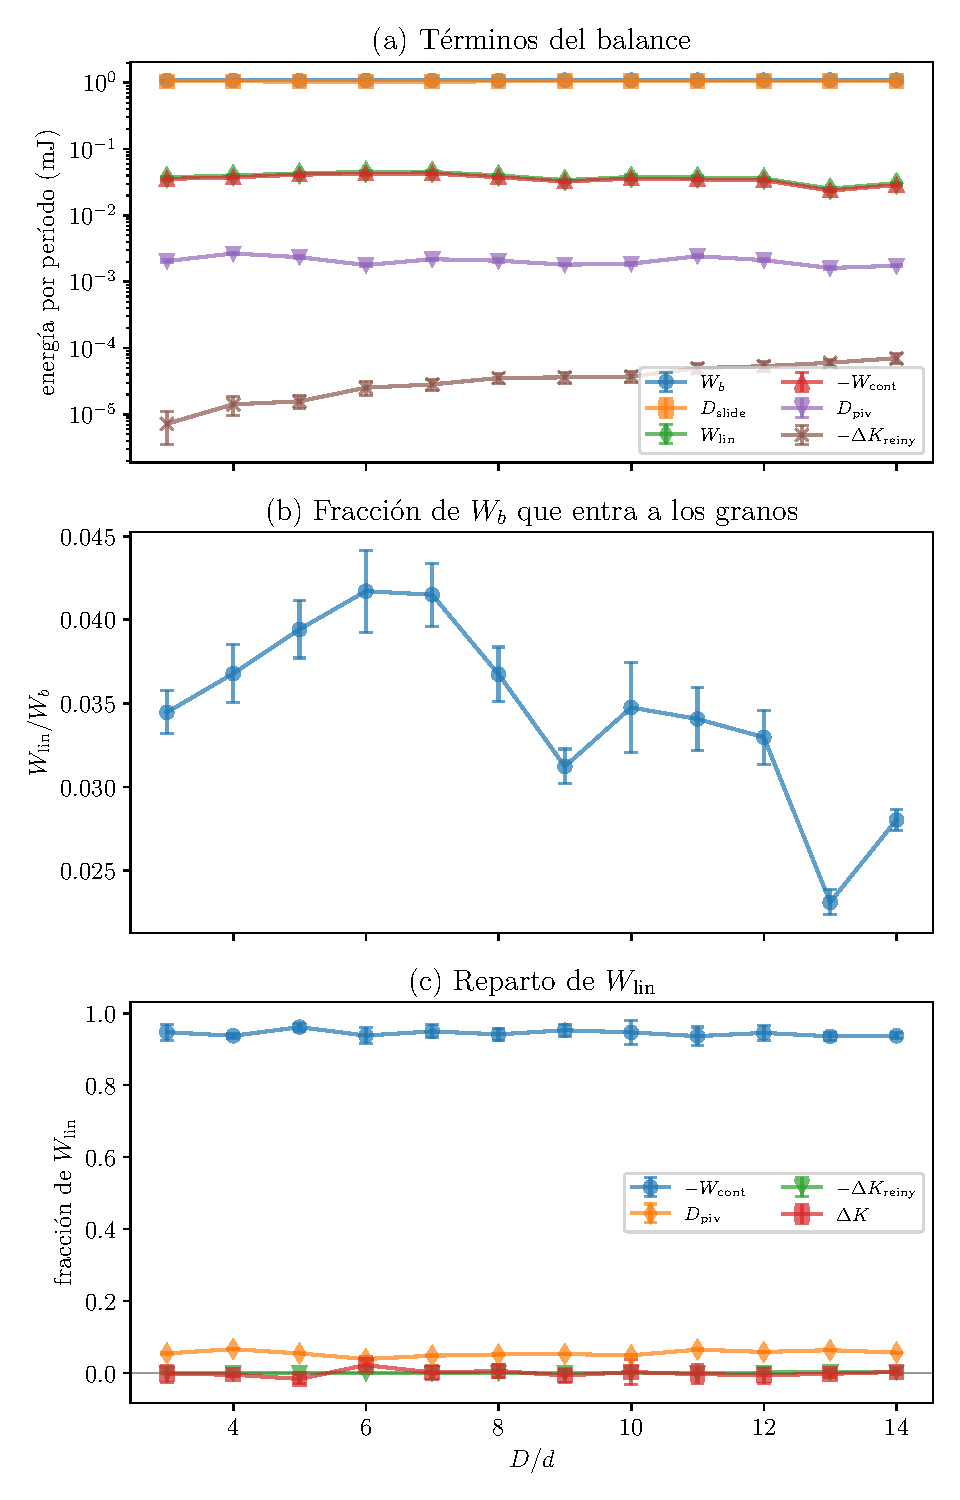
\includegraphics[width=0.62\textwidth]{figuras/energia-D}
  \caption{Balance por período en función de $D$ (\code{energia-D.pdf}).
    (a) Términos del balance, escala logarítmica. (b) Fracción de $\Wb$ que
    entra a los granos. (c) Reparto de $\Wlin$. Barras: error con bloques
    de dos períodos.}
  \label{fig:D}
\end{figure}

Las tablas~\ref{tab:balance} y~\ref{tab:fracciones} y la
figura~\ref{fig:D} resumen el balance. Cuatro hechos:
\begin{enumerate}
  \item El motor entrega $\Wb \approx 1.085$--$1.092$~mJ por período en
    todas las corridas, una potencia de $\approx 21.8$~mW para los 2000
    granos ($10.9~\mu$W por grano). Varía menos del 1\% con $D$.
  \item Casi todo se pierde deslizando contra la base: $\Dslide/\Wb =
    96$--$98\%$. Al medio granular entra solo $\Wlin/\Wb = 2.3$--$4.2\%$.
  \item De lo que entra, el reparto casi no depende de $D$: $\approx
    94\%$ se disipa en los contactos, 4--7\% en el pivoteo, y lo que se
    llevan los granos que salen es menos del 0.3\%.
  \item El cambio de $K$ por período es compatible con cero en todas las
    corridas: el registro es estacionario.
\end{enumerate}

\subsection{El trabajo de la base: granos casi quietos}
\label{sec:quietos}

Que $\Wb$ casi no dependa de $D$ tiene una explicación simple. Si los
granos estuvieran quietos, todos deslizarían contra la base todo el tiempo
y la fuerza de Karnopp sobre cada uno sería $\mu_d m g$ en el sentido de
$\vv_b$, así que
\begin{equation}
  \Wb^\text{quietos} = N_g\, \mu_d m g \ave{|v_b|}\, T
  = 2000 \times 0.13 \times 0.191 \times 2.214\ mgd = 110.2\ mgd =
  1.134\ \text{mJ} .
  \label{eq:quietos}
\end{equation}
El valor medido es el 95.6--96.3\% de esta cota en todas las corridas.
Los granos se mueven poco comparados con la base: la velocidad media de
deslizamiento, $\Dslide/(N_g \mu_d m g T) = 0.175$--$0.180\sqrt{gd}
\approx 3.9$~cm/s, es el 91--94\% de $\ave{|v_b|}$. La
figura~\ref{fig:base} muestra que esto vale también dentro del ciclo: el
trabajo de la base por unidad de fase sigue a $N_g \mu_d m g |v_b| T$
casi exactamente, salvo cerca de la fase 0.72, donde $v_b$ cambia de signo
rápido y los granos que estaban siendo arrastrados todavía se mueven con la
base.

Como consecuencia, $\Wb$ está fijado por la excitación y por $\mu_d$, no
por el estado del medio granular. Lo que depende de $D$ es la pequeña
fracción que entra a los granos.

\begin{figure}[ht]
  \centering
  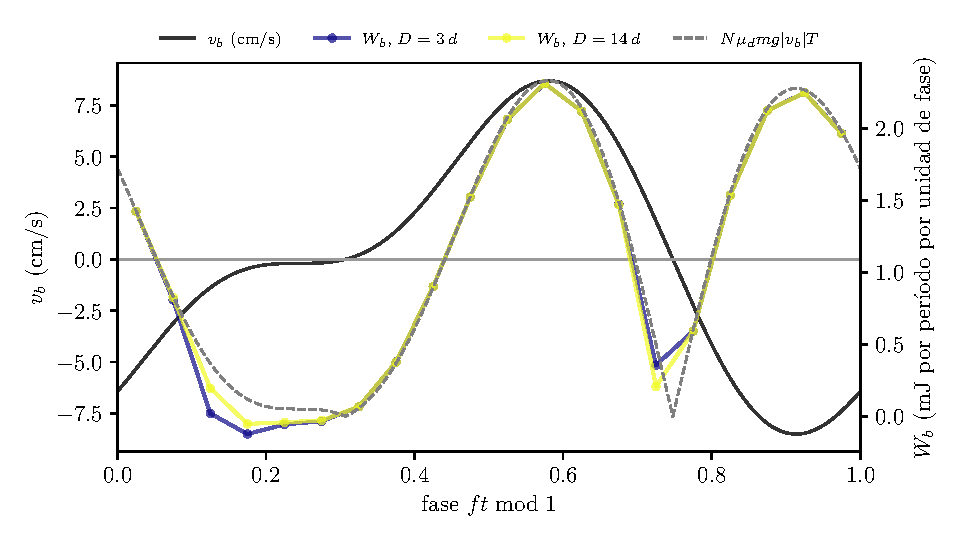
\includegraphics[width=0.75\textwidth]{figuras/base}
  \caption{Velocidad de la base en coordenadas experimentales (eje
    izquierdo) y trabajo de la base por período y por unidad de fase para
    $D = 3d$ y $14d$ (eje derecho), junto con el de granos quietos,
    $N_g \mu_d m g |v_b| T$ (trazos).}
  \label{fig:base}
\end{figure}

\subsection{Lo que entra a los granos}

$\Wlin/\Wb$ no es monótono en $D$ (figura~\ref{fig:D}b): crece de
$3.45(13)\%$ en $D = 3d$ a $\approx 4.2\%$ en $D = 6d$--$7d$ y luego
baja hasta $2.8\%$ en $D = 14d$. $D = 13d$ queda claramente por debajo de
sus vecinos, $2.31(7)\%$. Los errores son estadísticos dentro de cada
corrida; con una sola semilla no hay forma de separar una tendencia en $D$
de las diferencias entre corridas (por ejemplo, de la estructura de arcos
de cada una), así que esta dependencia hay que tomarla con cautela hasta
tener réplicas.

La figura~\ref{fig:fase} muestra dónde ocurre cada cosa dentro del ciclo.
$\Wlin$ es positivo en dos ventanas, en las que la base arrastra a los
granos (fases $\approx 0.37$--$0.7$ y $\approx 0.92$--$0.1$), y negativo
en otras dos, en las que la base cambia de sentido y los frena (fases
$\approx 0.12$--$0.35$ y $0.72$--$0.9$): la base da y quita energía dentro
de cada ciclo, y $\Wlin$ es el neto, un 25--40\% de lo que entrega en
las ventanas positivas. Los contactos disipan casi todo entre las fases
$0.5$ y $0.85$, mientras la base acelera a los granos y $\ave{K}$ sube
hacia su máximo (fase $\approx 0.72$); fuera de esa ventana $\Wcont$ es
casi nulo. Ese máximo crece con $D$, de $\approx 42~\mu$J en $D = 3d$ a
$\approx 88~\mu$J en $D = 14d$. En los $D$ chicos $\ave{K}$ tiene un
segundo máximo, de tamaño parecido, en la fase $\approx 0.12$.

\begin{figure}[ht]
  \centering
  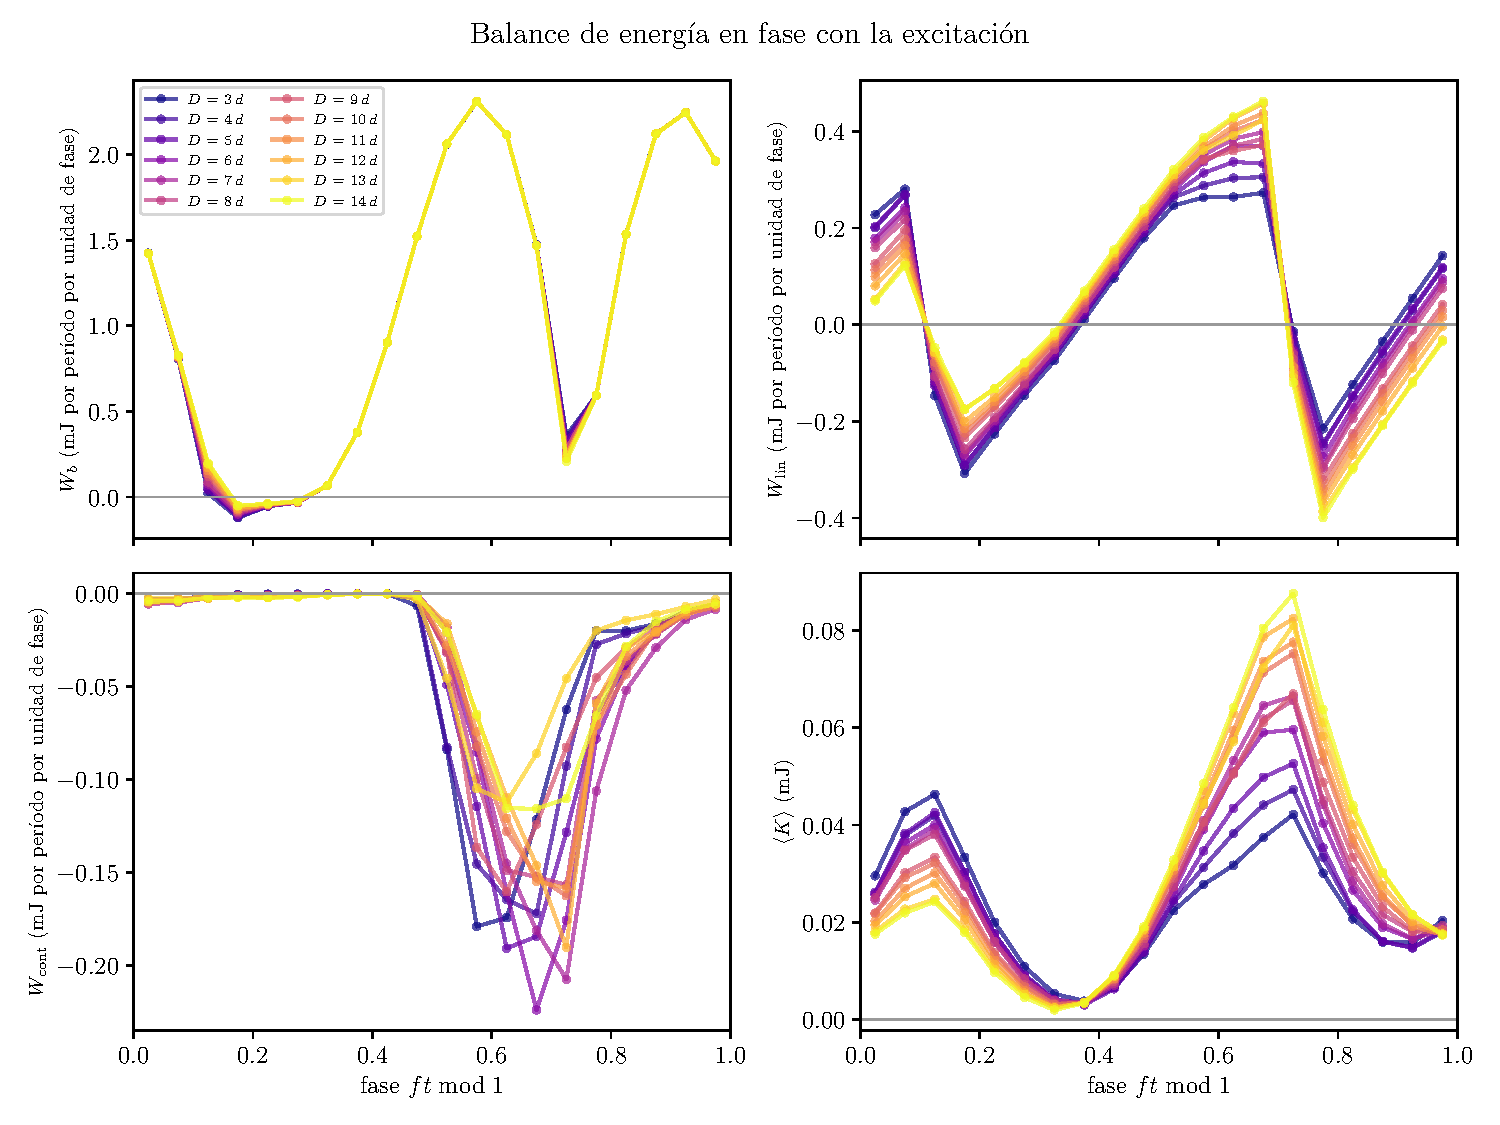
\includegraphics[width=\textwidth]{figuras/energia-fase}
  \caption{Balance en fase con la excitación (\code{energia-fase.pdf}):
    trabajo por período y por unidad de fase de la base, de la fricción y
    de los contactos, y energía cinética media.}
  \label{fig:fase}
\end{figure}

\subsection{Energía que sale por el orificio}

Dividiendo $-\dKr$ por el número de granos descargados en el registro
(de los archivos \code{flx-<NN>.dat}) se obtiene la energía cinética con que
cada grano llega a $y = -10$: $K_\text{sal} = 0.0032$--$0.0048\,mgd$, sin
tendencia con $D$, que equivale a una rapidez
$\sqrt{2K_\text{sal}/m} = 0.08$--$0.10\sqrt{gd} = 1.8$--$2.2$~cm/s.
Es el doble de la energía cinética media de los granos en el bin más bajo
del perfil de velocidad ($-10 < y < -9$ en \code{perfil-ve-<NN>.dat}):
$\ave{K} \approx 0.0020\,mgd$, rapidez media $0.050\sqrt{gd} =
1.1$~cm/s. La diferencia no es un error del balance sino de qué se
promedia. El perfil promedia los granos que están en el bin; el balance,
los que cruzan $y = -10$, y un grano rápido cruza antes que uno lento. Ese
promedio está pesado por el flujo, $\ave{|v_y| K}/\ave{|v_y|}$ sobre los
granos que bajan, y como debajo del orificio los granos siguen apoyados en
la base y oscilan con ella (el 17\,\% sube en cada instante), el peso
favorece las fases rápidas. Calculado con los \code{.ve} en
$-10.5 < y < -9$, el promedio pesado por el flujo da $0.0035$--$0.0036\,mgd$
para $D = 3d$, $10d$ y $14d$, de acuerdo con el balance dentro de la
estadística (en el registro salen 5 granos para $D = 3d$ y 49 para
$D = 14d$).
El número de granos que salen por período va de 0.17 ($D = 3d$) a 1.7
($D = 14d$), así que $-\dKr$ crece con $D$ como el caudal, pero sigue siendo
como mucho $2 \times 10^{-3}$ de $\Wlin$: la energía que se lleva el flujo de
descarga es despreciable en el balance.

\subsection{Respuesta de período 2}
\label{sec:periodo2}

Las series período a período (figuras~\ref{fig:periodos}
y~\ref{fig:alternancia}) muestran que $\Wb$, $\Wlin$, $\Wcont$ y $\ave{K}$
alternan entre un valor alto y uno bajo de un período al siguiente. La
autocorrelación entre períodos consecutivos,
\[
  r_1 = \frac{\sum_n \delta x_n\, \delta x_{n+1}}{\sum_n \delta x_n^2} ,
  \qquad \delta x_n = x_n - \bar x ,
\]
es fuertemente negativa (tabla~\ref{tab:alternancia}). En $D = 3d$ la
alternancia es tan grande que $\Wlin$ es negativo en uno de cada dos
períodos: en esos períodos la base le quita energía al medio granular. En
$D = 12d$ y $14d$ es mucho más débil ($r_1 \approx -0.6$). En $D = 7d$ se
ve un cambio de paridad alrededor del período 5: la alternancia se
interrumpe y se retoma corrida en un período.

\begin{table}[ht]
\centering
\small
\caption{Alternancia período a período. $r_1$: autocorrelación entre
  períodos consecutivos. $A = \ave{|W_{\text{lin},n+1} - W_{\text{lin},n}|}
  / (2 \ave{\Wlin})$: semiamplitud de la alternancia de $\Wlin$ relativa a
  su media.}
\label{tab:alternancia}
\begin{tabular}{rrrrr}
  \toprule
  $D/d$ & $r_1(\Wb)$ & $r_1(\Wlin)$ & $r_1(\ave{K})$ & $A$ \\
  \midrule
  3 & $-0.96$ & $-0.95$ & $-0.95$ & 2.25 \\
  4 & $-0.95$ & $-0.95$ & $-0.94$ & 1.71 \\
  5 & $-0.92$ & $-0.94$ & $-0.88$ & 1.32 \\
  6 & $-0.90$ & $-0.91$ & $-0.85$ & 1.16 \\
  7 & $-0.93$ & $-0.91$ & $-0.75$ & 0.86 \\
  8 & $-0.92$ & $-0.94$ & $-0.84$ & 1.46 \\
  9 & $-0.95$ & $-0.97$ & $-0.93$ & 1.49 \\
  10 & $-0.85$ & $-0.86$ & $-0.80$ & 0.71 \\
  11 & $-0.80$ & $-0.83$ & $-0.77$ & 0.65 \\
  12 & $-0.57$ & $-0.60$ & $-0.34$ & 0.28 \\
  13 & $-0.95$ & $-0.95$ & $-0.91$ & 1.72 \\
  14 & $-0.58$ & $-0.68$ & $-0.47$ & 0.22 \\
  \bottomrule
\end{tabular}
\end{table}

La excitación es periódica de período $T$ (el segundo armónico tiene
período $T/2$), así que una respuesta de período $2T$ es subarmónica: la
rompe espontáneamente el medio granular. La sección~\ref{sec:paridad}
muestra que el lecho alterna entre dos ciclos de naturaleza distinta. Que $D = 13d$, la corrida con $\Wlin/\Wb$ más bajo, tenga una de
las alternancias más fuertes, y que $D = 12d$ y $14d$ tengan las más
débiles, sugiere que el estado de cada corrida pesa en el balance tanto
como $D$.

Para el análisis estadístico la consecuencia es directa: con $r_1 \approx
-0.9$ los períodos no son independientes. Con bloques de un período los
errores salían entre 3 y 10 veces más grandes que con bloques de dos (la
alternancia se cuenta como ruido), y con bloques de cuatro casi no cambian
respecto de dos. Por eso \code{plot-energia.py} usa bloques de dos períodos.

\begin{figure}[ht]
  \centering
  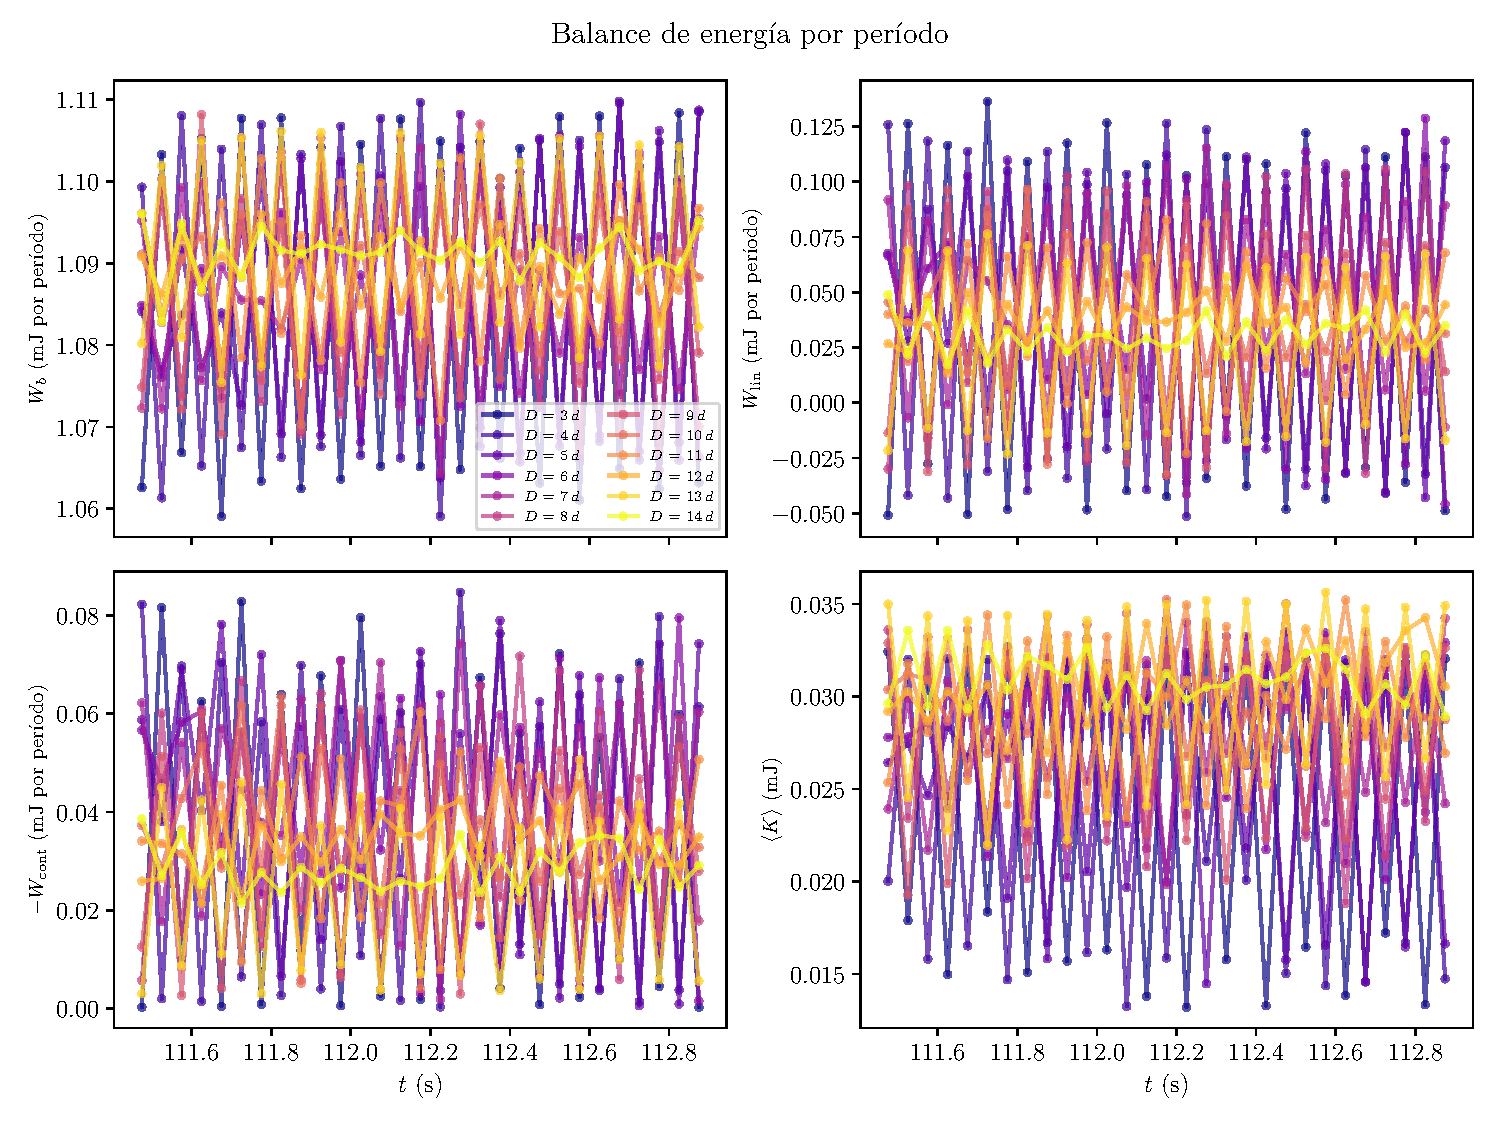
\includegraphics[width=\textwidth]{figuras/energia-periodos}
  \caption{Series período a período (\code{energia-periodos.pdf}).}
  \label{fig:periodos}
\end{figure}

\begin{figure}[ht]
  \centering
  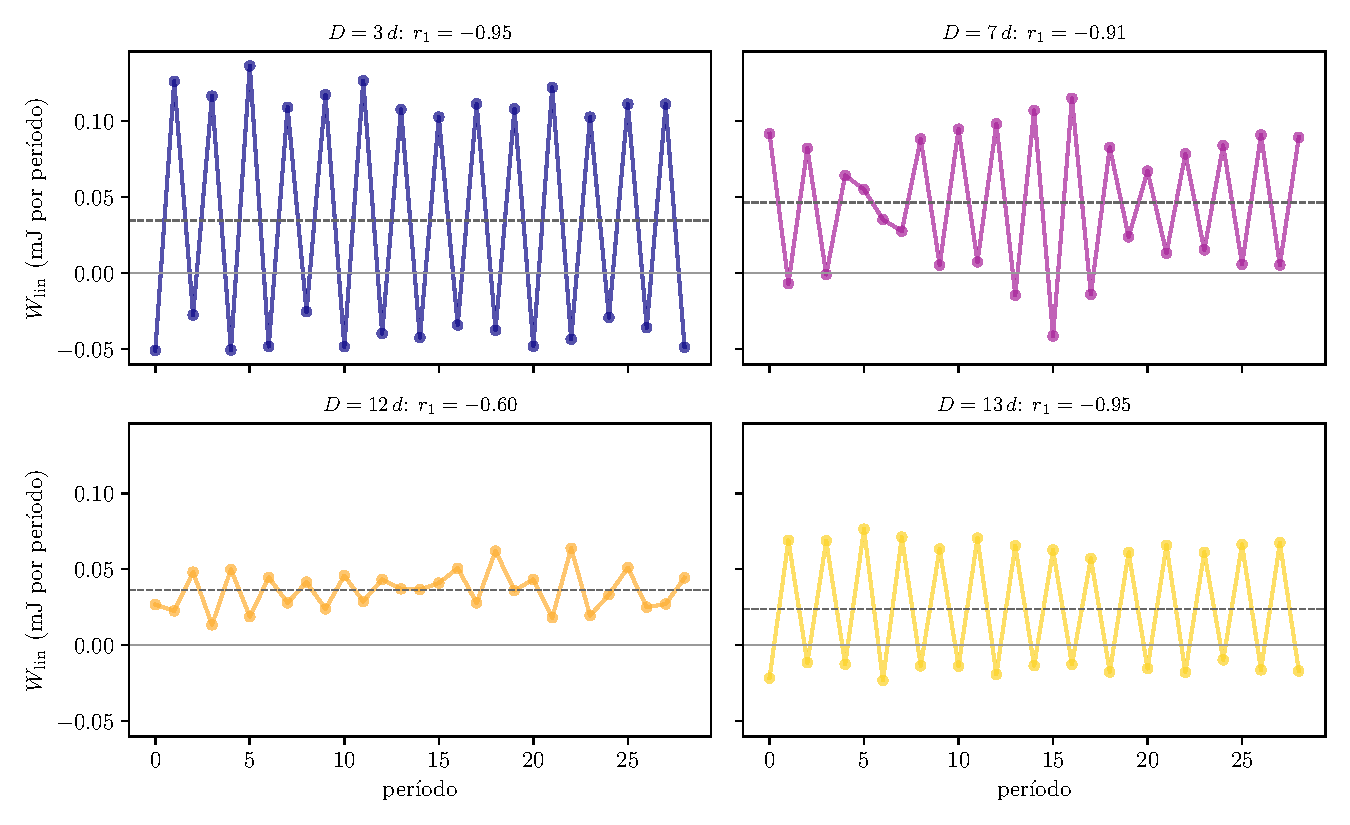
\includegraphics[width=0.9\textwidth]{figuras/alternancia}
  \caption{$\Wlin$ por período para cuatro orificios. Trazos: media.
    $r_1$: autocorrelación entre períodos consecutivos.}
  \label{fig:alternancia}
\end{figure}

\subsection{Períodos pares e impares}
\label{sec:paridad}

\code{tools/scripts/plot-energia-paridad.py} separa los períodos completos
según la paridad de $b = \lfloor f t \rfloor$. Los totales por período
salen directamente de \code{energy\_<pre>.dat}. En fase, en cambio, el
archivo del simulador suma todos los períodos, así que solo se puede
separar la energía cinética, que se reconstruye con los \code{.ve}: cada
frame se asigna a su período por $t$ y a su bin por la fase de la
cabecera. Los trabajos en fase separados por paridad requieren una salida
nueva del simulador (sección de pendientes).

Qué paridad es la alta depende de cuándo empieza el registro, así que las
figuras comparan el período de $\Wlin$ alto con el de $\Wlin$ bajo de cada
corrida. La coherencia, la fracción de pares de períodos consecutivos en
que el de la paridad alta tiene más $\Wlin$, vale 1 en seis corridas,
0.93--0.96 en cuatro y 0.82 en $D = 12d$ y $14d$: la alternancia está
trabada a la paridad durante todo el registro, salvo uno o dos saltos.

\begin{table}[ht]
\centering
\small
\caption{Medias en los períodos de $\Wlin$ alto y bajo, en $\mu$J
  (error estándar entre los 14 o 15 períodos de cada paridad).}
\label{tab:paridad}
\begin{tabular}{rcc rr rr rr}
  \toprule
  & & & \multicolumn{2}{c}{$\Wlin$} & \multicolumn{2}{c}{$-\Wcont$} &
    \multicolumn{2}{c}{$\ave{K}$} \\
  \cmidrule(lr){4-5} \cmidrule(lr){6-7} \cmidrule(lr){8-9}
  $D/d$ & alta & coher. & alto & bajo & alto & bajo & alto & bajo \\
  \midrule
  3 & par & 1.00 & 115(3) & $-41(2)$ & 67(3) & 4(1) & 15.4(5) & 32.2(1) \\
  4 & impar & 1.00 & 112(3) & $-33(3)$ & 69(2) & 6(2) & 16.4(6) & 31.8(1) \\
  5 & impar & 1.00 & 103(3) & $-16(6)$ & 68(2) & 15(4) & 19.3(11) & 31.1(4) \\
  6 & par & 0.93 & 90(6) & $-3(9)$ & 62(2) & 21(5) & 22.9(6) & 31.5(5) \\
  7 & impar & 0.96 & 85(5) & 6(6) & 61(2) & 25(3) & 24.7(6) & 31.3(4) \\
  8 & par & 1.00 & 96(3) & $-16(3)$ & 62(2) & 14(2) & 23.0(6) & 32.6(2) \\
  9 & par & 1.00 & 84(3) & $-14(3)$ & 54(2) & 12(2) & 22.2(4) & 33.0(2) \\
  10 & par & 0.93 & 62(6) & 15(6) & 47(3) & 25(3) & 26.8(5) & 32.0(5) \\
  11 & impar & 0.96 & 62(4) & 13(5) & 46(2) & 24(3) & 26.1(5) & 33.0(4) \\
  12 & impar & 0.82 & 44(3) & 28(3) & 37(2) & 30(2) & 28.9(5) & 32.0(4) \\
  13 & par & 1.00 & 66(1) & $-16(1)$ & 41(1) & 6(1) & 24.4(4) & 34.8(1) \\
  14 & impar & 0.82 & 37(2) & 24(1) & 31(1) & 26(1) & 30.6(3) & 31.4(4) \\
  \bottomrule
\end{tabular}
\end{table}

La tabla~\ref{tab:paridad} y las figuras~\ref{fig:paridadD}
y~\ref{fig:paridadfase} muestran que los dos ciclos son de naturaleza
distinta:
\begin{itemize}
  \item En el ciclo de $\Wlin$ \emph{alto} la base inyecta mucha energía
    (hasta $115~\mu$J por período en $D = 3d$, tres veces la media), los
    contactos disipan casi toda, y la energía cinética es baja.
  \item En el ciclo de $\Wlin$ \emph{bajo} la energía cinética es alta, los
    contactos casi no disipan (4--6~$\mu$J en $D = 3d$, $4d$ y $13d$), y la
    base le \emph{quita} energía al lecho: $\Wlin < 0$ en siete de las doce
    corridas.
\end{itemize}
En fase (figura~\ref{fig:paridadfase}), el ciclo de $\Wlin$ bajo tiene dos
máximos de $\ave{K}$ grandes, en la fase $\approx 0.1$ y en la
$\approx 0.7$, de hasta 0.08--0.10~mJ; el de $\Wlin$ alto tiene los mismos
máximos mucho más chicos. Una lectura compatible con esto: en el ciclo de
$\Wlin$ bajo los granos se mueven juntos, arrastrados por la base, con
mucha energía cinética pero pocas colisiones, y la base los frena al
cambiar de sentido; en el siguiente, el lecho no acompaña a la base, que
lo agita, y la energía se disipa en los contactos. Separar los trabajos en
fase por paridad permitiría confirmarlo.

El contraste disminuye con $D$: $\ave{K}$ del ciclo bajo es $\approx
32~\mu$J en todas las corridas, mientras que el del ciclo alto sube de 15
a 31~$\mu$J. En $D = 14d$ los dos ciclos casi coinciden.

\begin{figure}[ht]
  \centering
  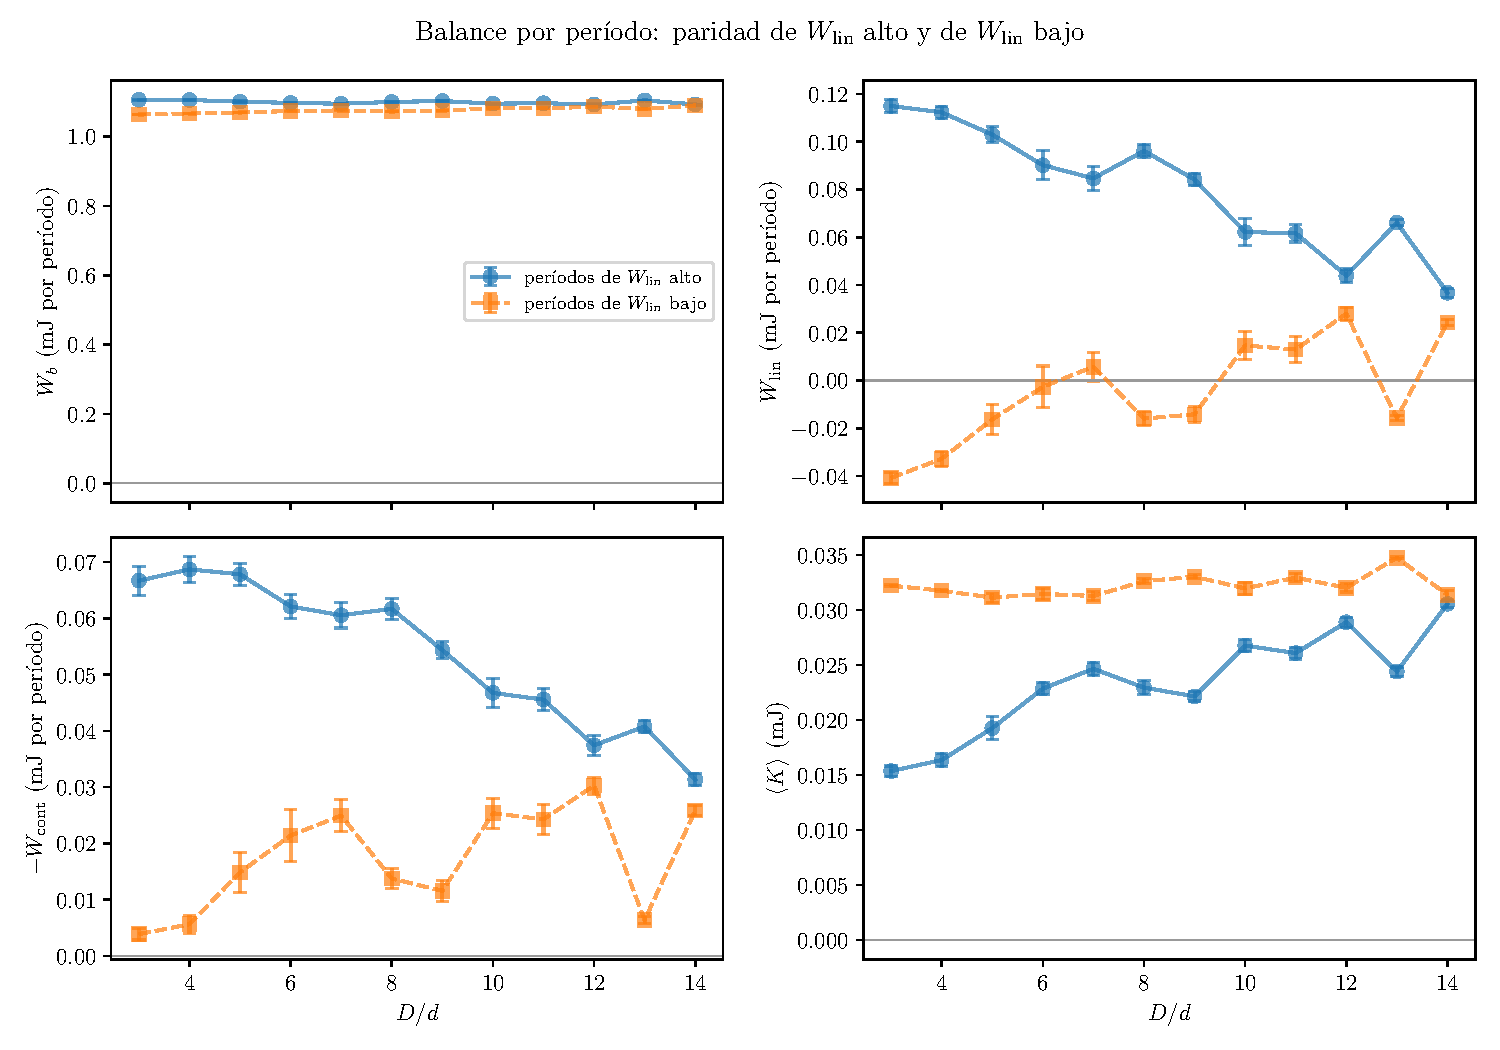
\includegraphics[width=\textwidth]{figuras/energia-paridad-D}
  \caption{Medias por período en los ciclos de $\Wlin$ alto (línea) y bajo
    (trazos), en función de $D$ (\code{energia-paridad-D.pdf}).}
  \label{fig:paridadD}
\end{figure}

\begin{figure}[ht]
  \centering
  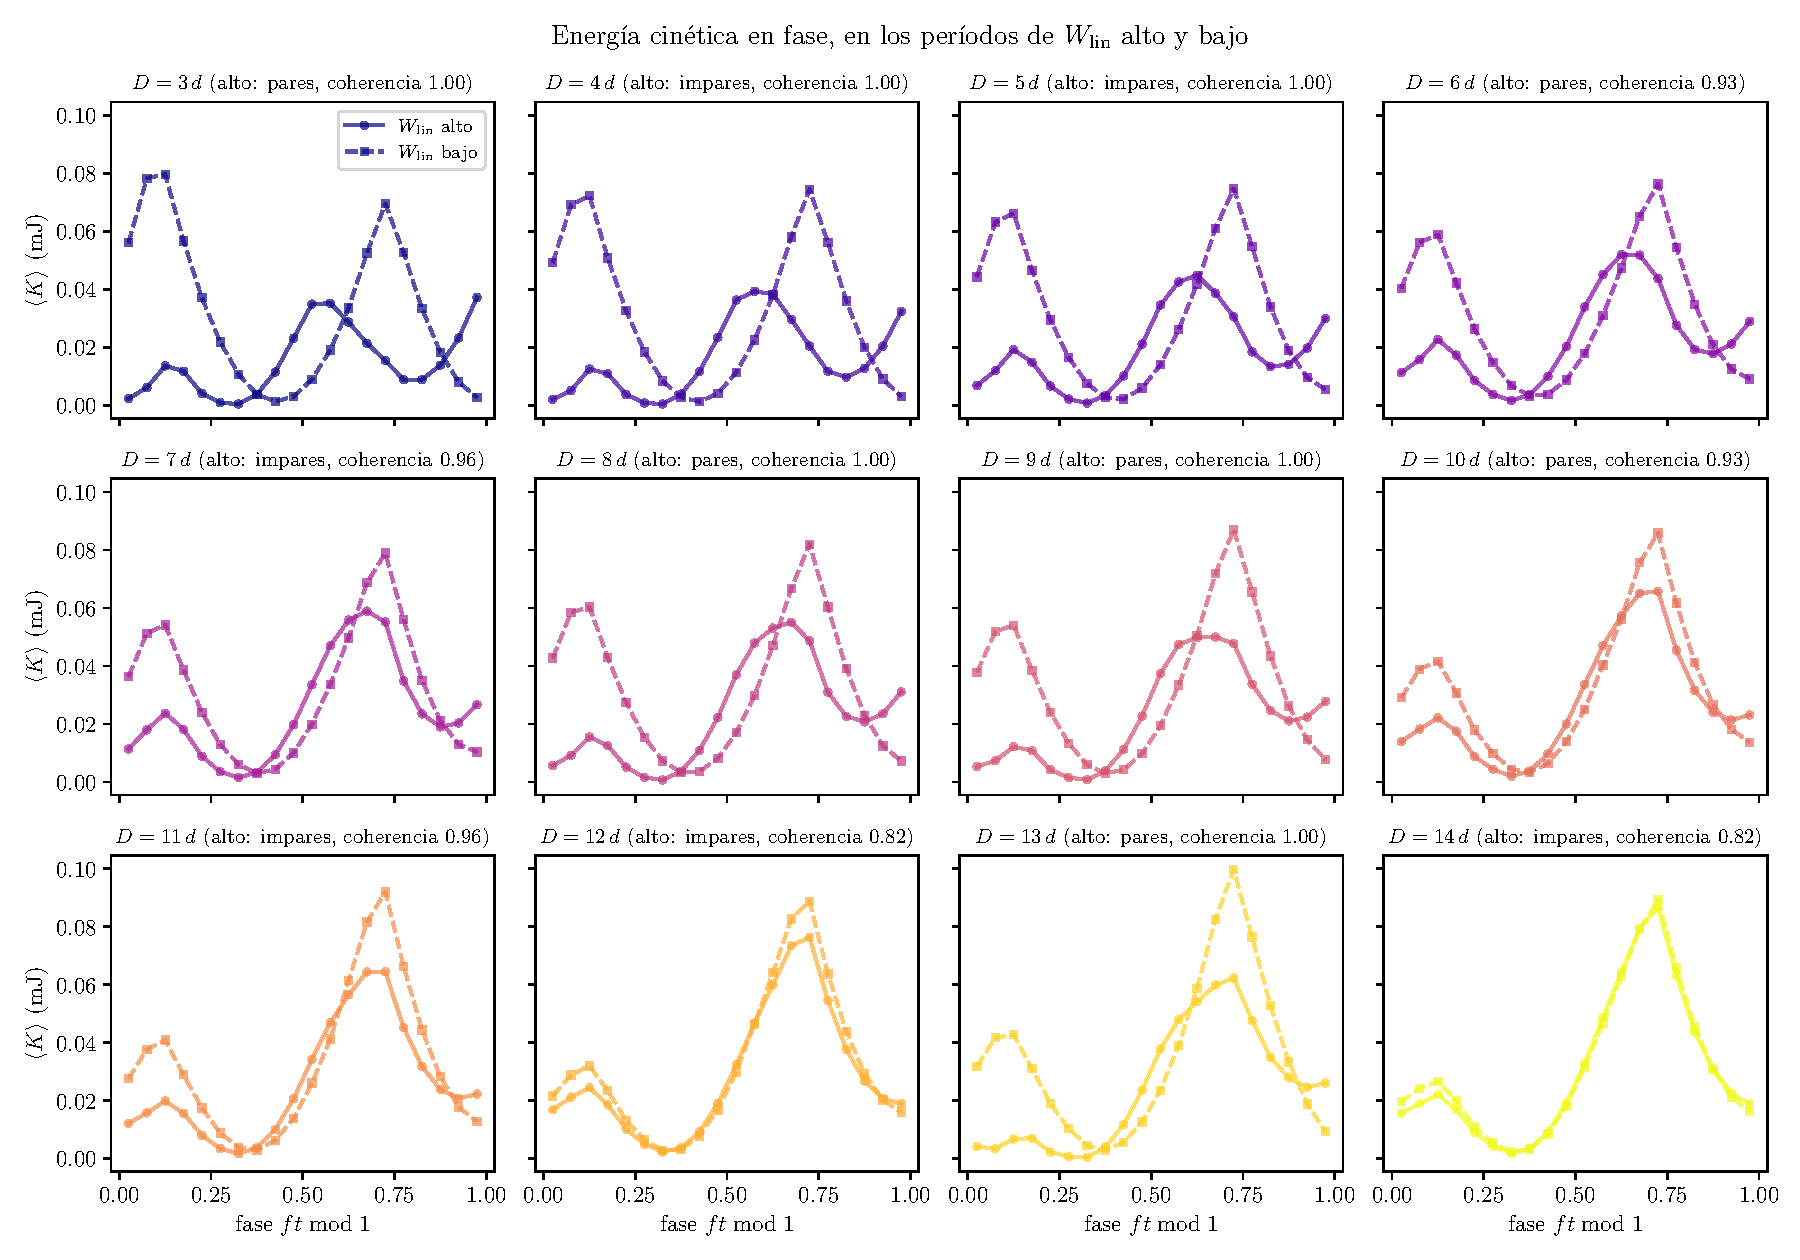
\includegraphics[width=\textwidth]{figuras/energia-paridad-fase}
  \caption{Energía cinética total en fase en los ciclos de $\Wlin$ alto
    (línea) y bajo (trazos), de los \code{.ve}
    (\code{energia-paridad-fase.pdf}). Entre paréntesis, la paridad del
    ciclo alto y la coherencia.}
  \label{fig:paridadfase}
\end{figure}

% ---------------------------------------------------------------------------
\section{Relación con la propuesta original}

La medición se diseñó a partir del análisis del 23 de octubre de 2026
(perfiles de fuerza, velocidad y energía, que no está en el repositorio).
Respecto de esa propuesta:
\begin{itemize}
  \item Se confirma la estimación de que $\Wb$ es mucho mayor que lo que
    entra a los granos: $\Wg/\Wb \approx 3\%$.
  \item El trabajo de la primera etapa del paso, (\ref{eq:wlin}), es el de
    la propuesta, pero reconstruido con la aritmética de Box2D para que el
    cierre sea exacto.
  \item La foto de las velocidades se toma justo antes de \code{Step},
    después de la reinyección, en lugar de registrarla al aplicar la
    fricción. Así no quedan punteros a cuerpos movidos ni velocidades
    viejas (supuesto~2 de la propuesta).
  \item La energía de la descarga y la reinyección, que la propuesta
    dejaba fuera del balance, se mide como $\dKr$, y el balance
    (\ref{eq:cierre}) cierra sin residuo.
\end{itemize}

% ---------------------------------------------------------------------------
\section{Pendientes}

\begin{itemize}
  \item Período 2: guardar el balance en fase de cada período (o por
    paridad) en el simulador, para separar $\Wb$, $\Wlin$ y $\Wcont$ en
    fase; separar también los perfiles por paridad; verificar con registros
    más largos y otras semillas.
  \item Réplicas con otras semillas para decidir si la dependencia de
    $\Wlin/\Wb$ con $D$ (máximo en $D \approx 6d$--$7d$, mínimo en $13d$)
    es una tendencia o una diferencia entre corridas.
  \item Relacionar el máximo de $\ave{K}$ en fase con la oscilación
    coherente de los granos (perfiles en fase de \code{stress\_profile}).
\end{itemize}

\end{document}
